\chapter{Kernel Ridge Regression}

\section{Introduction to the regression problem}

In this section we introduce the regression problem that will be used throughout the project. Assume we have a dataset $(x_i,y_i)$ for $i=1,\ldots,n$ where $x_i\in\mathbb{R}^d$ are inputs and $y_i\in\mathbb{R}$ are outputs. We would like to use these data to create a model for the relationship between the $x$ and $y$. In ordinary linear regression one searches over linear functions of the input variables. Kernel ridge regression instead searches over a reproducing kernel Hilbert space $\mathcal{H}$, which allows nonlinear functions to be represented through a kernel function.

Let
\[
k:\mathbb{R}^d\times\mathbb{R}^d\to\mathbb{R}
\]
be a positive definite kernel function. For the training data we define the kernel matrix
\[
K\in\mathbb{R}^{n\times n},\quad K_{ij}=k(x_i,x_j).
\]
The entry $K_{ij}$ measures the similarity between the data points $x_i$ and $x_j$ according to the chosen kernel function. The matrix $K$ induced by $k$ is symmetric positive semidefinite.

The kernel trick allows us to formulate this as
\[
\min_{f\in\mathcal{H}}\|f(X)-y\|_2^2+\lambda\|f\|_{\mathcal{H}}^2,
\]
which is also
\[
\min_{f\in\mathcal{H}}\sum_{i=1}^n(f(x_i)-y_i)^2+\lambda\|f\|_{\mathcal{H}}^2.
\]
Here $\lambda>0$ is the regularization parameter. The first term measures the error on the training data while the second term penalizes functions with large RKHS norm. Here $\lambda$ controls the trade off between fitting the data and overfitting.

\section{Representer form}

By the representer theorem, the minimizer has the form
\[
f(x)=\sum_{j=1}^n\alpha_j k(x,x_j),
\]
for some coefficient vector
\[
\alpha=(\alpha_1,\ldots,\alpha_n)^T\in\mathbb{R}^n.
\]
For the training points we have
\[
f(x_i)=\sum_{j=1}^n\alpha_j k(x_i,x_j),
\]
so in vector form
\[
f(X)=K\alpha.
\]
Therefore the data fitting term becomes
\[
\sum_{i=1}^n(f(x_i)-y_i)^2=\|K\alpha-y\|_2^2.
\]

The RKHS norm term can also be written using the kernel matrix. First, by the reproducing property,
\[
\langle k(\cdot,x_i),k(\cdot,x_j)\rangle_{\mathcal{H}}=k(x_i,x_j).
\]
Since
\[
f=\sum_{i=1}^n\alpha_i k(\cdot,x_i),
\]
we have
\[
\|f\|_{\mathcal{H}}^2=\left\langle\sum_{i=1}^n\alpha_i k(\cdot,x_i),\sum_{j=1}^n\alpha_j k(\cdot,x_j)\right\rangle_{\mathcal{H}}.
\]
Using bilinearity of the inner product,
\[
\|f\|_{\mathcal{H}}^2=\sum_{i=1}^n\sum_{j=1}^n\alpha_i\alpha_j\langle k(\cdot,x_i),k(\cdot,x_j)\rangle_{\mathcal{H}}.
\]
Using the reproducing property again,
\[
\|f\|_{\mathcal{H}}^2=\sum_{i=1}^n\sum_{j=1}^n\alpha_i\alpha_j k(x_i,x_j).
\]
Since $K_{ij}=k(x_i,x_j)$ this becomes
\[
\|f\|_{\mathcal{H}}^2=\alpha^T K\alpha.
\]
Substituting this into the objective gives
\[
\min_{\alpha\in\mathbb{R}^n}\|K\alpha-y\|_2^2+\lambda\alpha^T K\alpha.
\]
Expand
\[
\|K\alpha-y\|_2^2=(K\alpha-y)^T(K\alpha-y).
\]
Then differentiate
\[
(K\alpha-y)^T(K\alpha-y)+\lambda\alpha^T K\alpha
\]
with respect to $\alpha$. Since $K$ is symmetric this gives
\[
2K(K\alpha-y)+2\lambda K\alpha=0.
\]
This then reduces to
\[
(K+\lambda I)\alpha=y.
\]
Therefore the coefficient vector is
\[
\alpha=(K+\lambda I)^{-1}y.
\]
The prediction for a new point $x$ is then
\[
\hat f(x)=\sum_{j=1}^n\alpha_j k(x,x_j).
\]
If $X_{\text{test}}$ is a set of test points and $K_{\text{test},\text{train}}$ is the matrix with entries
\[
(K_{\text{test},\text{train}})_{ij}=k(x_i^{\text{test}},x_j^{\text{train}}),
\]
then the test predictions are
\[
\hat y_{\text{test}}=K_{\text{test},\text{train}}\alpha.
\]

The regularization term is important numerically. Since $K$ can have very small eigenvalues or even zero eigenvalues, adding $\lambda I$ shifts all eigenvalues by $\lambda$ so $K+\lambda I$ is positive definite. This makes the system uniquely solvable and improves the conditioning of the problem.

For large datasets, the main computational difficulty is that $K$ is an $n\times n$ matrix. Forming the full kernel matrix requires $O(n^2)$ kernel evaluations and storing it requires $O(n^2)$ memory. Solving the system directly, for example by Cholesky decomposition, costs $O(n^3)$ operations. For small $n$ this is fine but for large datasets this quickly becomes infeasible. Therefore in this project we investigate the Nystr\"om approximation of the kernel matrix: instead of forming all of $K$, we only form $l\ll n$ sampled columns and the corresponding $l\times l$ submatrix, and then make a low rank approximation $\tilde K\approx K$.

\section{Kernel choices}

In the experiments we start with three common kernels. The linear kernel is
\[
k(x,z)=x^Tz.
\]
The polynomial kernel used in the first tests is
\[
k(x,z)=(x^Tz+1)^2.
\]
The Gaussian radial basis function kernel (rbf) is
\[
k(x,z)=\exp(-\gamma\|x-z\|_2^2).
\]
The parameter $\gamma$ controls how local the Gaussian kernel is. Larger $\gamma$ makes points only strongly similar to very nearby points while smaller $\gamma$ makes the similarities decay more slowly.

\section{Singular values and low-rank structure}

A kernel matrix is useful for Nystr\"om approximation when its singular values decay. If many singular values are very small then much of the matrix can be approximated using a smaller rank. This is why in this section we look at singular values of $K$ for real data. The point is to check whether a low-rank approximation is reasonable for real world data.

For this real data experiment we use the Superconductivity dataset from the UCI Machine Learning Repository. This is a regression dataset with $21263$ samples and $81$ numerical input features, and the output is the critical temperature. This fits the KRR setting since the target variable is continuous.

This dataset is also large enough to show the computational problem. If the full dataset is used, the kernel matrix has size
\[
21263\times 21263.
\]
This means there are
\[
21263^2=452115169
\]
entries in $K$. If these entries are stored in double precision, then just storing one dense kernel matrix takes about
\[
452115169\cdot 8\text{ bytes}\approx 3.6\text{ GB}.
\]
This is before solving the linear system or computing any decomposition. So the full matrix is already expensive, and this is the reason that an approximation method such as Nystr\"om is relevant.

The first singular value experiment uses the linear kernel
\[
k(x,z)=x^Tz.
\]
For a data matrix $X\in\mathbb{R}^{n\times d}$, this gives
\[
K=XX^T.
\]
In the Superconductivity dataset $d=81$, so the linear kernel matrix satisfies
\[
\operatorname{rank}(K)\leq 81.
\]
Therefore for the linear kernel, at most $81$ singular values can be nonzero. This is a simple case where the low-rank structure is built into the kernel matrix. It is still a useful first check because it shows directly how the dimension of the data can limit the rank of $K$.

\begin{figure}[h]
\centering
\IfFileExists{Results/sing_vals_linear_kernel.pdf}{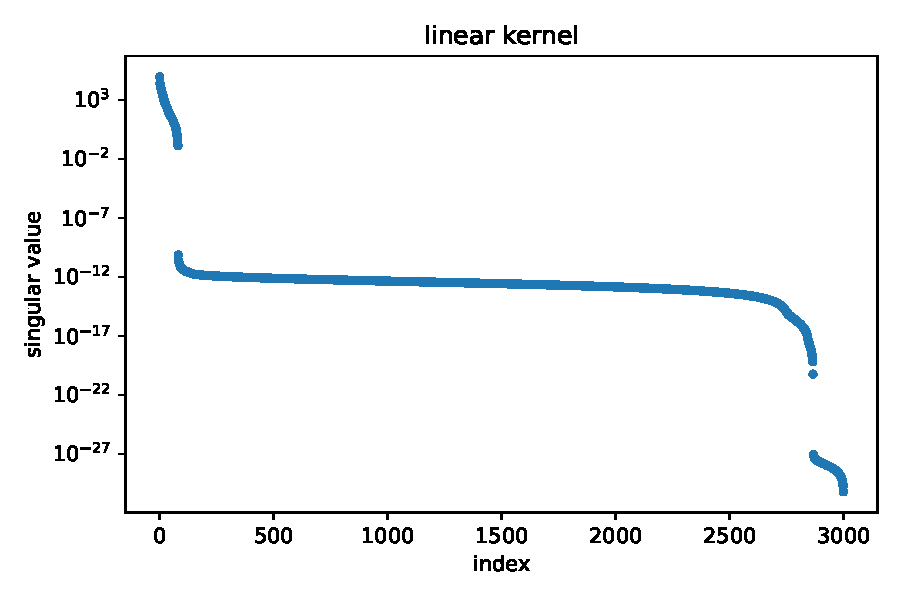
\includegraphics[width=0.75\textwidth]{Results/sing_vals_linear_kernel.pdf}}{\fbox{Run the singular value experiment to create this figure}}
\caption{Singular values of a kernel matrix from the Superconductivity dataset using the linear kernel.}
\label{fig:singular-linear}
\end{figure}

I also compare this with the Gaussian RBF kernel
\[
k(x,z)=\exp(-\gamma\|x-z\|_2^2).
\]
For this kernel the rank is not limited by $d$ in the same simple way. The singular value decay depends on the geometry of the data and on the parameter $\gamma$. This makes the RBF kernel more interesting for checking whether the singular values still decay in practice.

\begin{figure}[h]
\centering
\IfFileExists{Results/sing_vals_rbf_kernel.pdf}{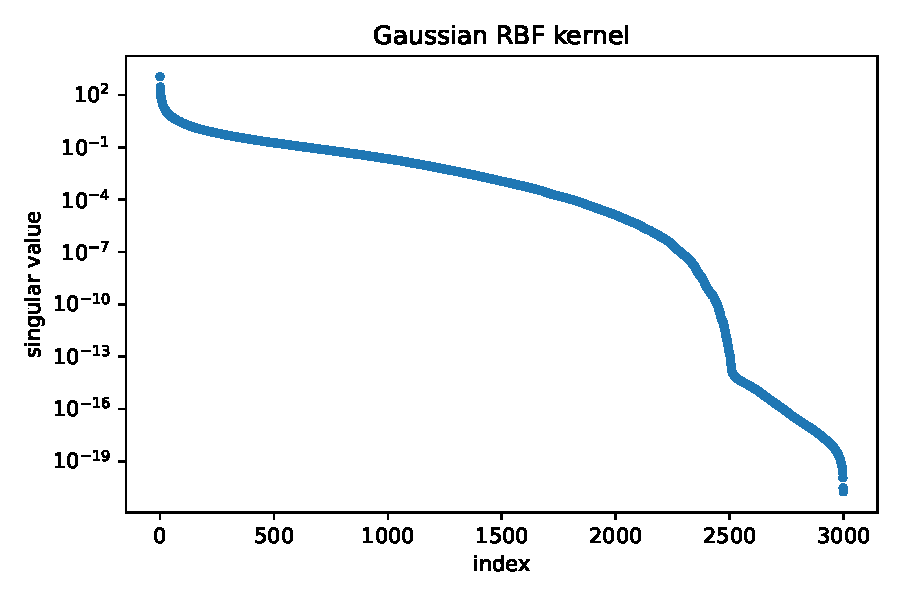
\includegraphics[width=0.75\textwidth]{Results/sing_vals_rbf_kernel.pdf}}{\fbox{Run the singular value experiment to create this figure}}
\caption{Singular values of a kernel matrix from the Superconductivity dataset using the Gaussian RBF kernel.}
\label{fig:singular-rbf}
\end{figure}